\documentclass[tikz,border=5pt]{standalone}
\usepackage[T1]{fontenc}
\usepackage{lmodern,amsmath,amssymb}
\usetikzlibrary{arrows.meta,calc,positioning,fit,backgrounds,shapes.geometric,matrix,decorations.pathreplacing,patterns}
\definecolor{ink}{gray}{0.08}
\definecolor{wash}{gray}{0.965}
\definecolor{soft}{gray}{0.45}
\tikzset{box/.style={draw=ink,line width=.65pt,fill=white,align=center,inner sep=4pt,outer sep=0pt,font=\small},flow/.style={draw=ink,line width=.65pt,-{Latex[length=1.8mm,width=1.3mm]},rounded corners=2pt},annotation/.style={font=\scriptsize,text=soft,align=center},groupbox/.style={draw=soft,dashed,line width=.45pt,fill=wash}}
\begin{document}
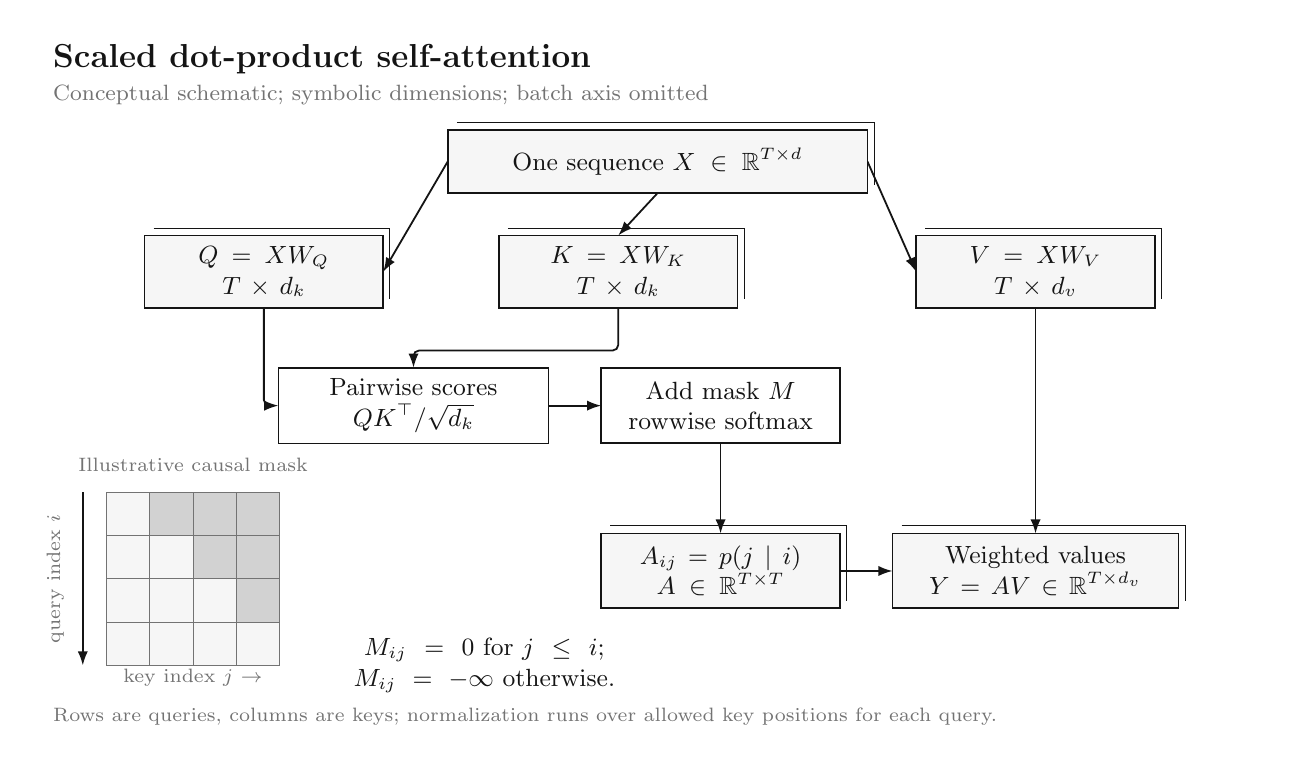
\begin{tikzpicture}[x=1cm,y=-1cm,font=\rmfamily,text=ink]

\path[use as bounding box] (0,0) rectangle (16,9);
\node[anchor=west,font=\large\bfseries] at (.2,.4) {Scaled dot-product self-attention};
\node[anchor=west,font=\footnotesize,text=soft] at (.2,.85) {Conceptual schematic; symbolic dimensions; batch axis omitted};
\begin{pgfonlayer}{background}
\end{pgfonlayer}
\node[box,fill=wash,minimum width=5.3cm,minimum height=0.8cm,text width=5.05cm] (x) at (8,1.7) {One sequence $X\in\mathbb{R}^{T\times d}$};
\draw[ink,line width=.4pt] (5.449999999999999,1.1999999999999997) -- (10.75,1.1999999999999997) -- (10.75,2.0);
\node[box,fill=wash,minimum width=3cm,minimum height=0.9cm,text width=2.75cm] (q) at (3,3.1) {$Q=XW_Q$\\$T\times d_k$};
\draw[ink,line width=.4pt] (1.6,2.55) -- (4.6,2.55) -- (4.6,3.45);
\node[box,fill=wash,minimum width=3cm,minimum height=0.9cm,text width=2.75cm] (k) at (7.5,3.1) {$K=XW_K$\\$T\times d_k$};
\draw[ink,line width=.4pt] (6.1,2.55) -- (9.1,2.55) -- (9.1,3.45);
\node[box,fill=wash,minimum width=3cm,minimum height=0.9cm,text width=2.75cm] (v) at (12.8,3.1) {$V=XW_V$\\$T\times d_v$};
\draw[ink,line width=.4pt] (11.4,2.55) -- (14.4,2.55) -- (14.4,3.45);
\node[box,minimum width=3.4cm,minimum height=0.95cm,text width=3.15cm] (score) at (4.9,4.8) {Pairwise scores\\$QK^\top/\sqrt{d_k}$};
\node[box,minimum width=3.0cm,minimum height=0.95cm,text width=2.75cm] (softmax) at (8.8,4.8) {Add mask $M$\\rowwise softmax};
\node[box,fill=wash,minimum width=3.0cm,minimum height=0.95cm,text width=2.75cm] (a) at (8.8,6.9) {$A_{ij}=p(j\mid i)$\\$A\in\mathbb{R}^{T\times T}$};
\draw[ink,line width=.4pt] (7.4,6.325000000000001) -- (10.4,6.325000000000001) -- (10.4,7.275);
\node[box,fill=wash,minimum width=3.6cm,minimum height=0.95cm,text width=3.35cm] (y) at (12.8,6.9) {Weighted values\\$Y=AV\in\mathbb{R}^{T\times d_v}$};
\draw[ink,line width=.4pt] (11.1,6.325000000000001) -- (14.700000000000001,6.325000000000001) -- (14.700000000000001,7.275);
\node[align=center,inner sep=0pt,outer sep=0pt,font=\small,minimum width=5.2cm,minimum height=0.5cm,text width=4.95cm] (note8) at (5.8,8.1) {$M_{ij}=0$ for $j\leq i$; $M_{ij}=-\infty$ otherwise.};
\begin{pgfonlayer}{background}
\draw[flow] (x.west) -- (q.east);
\draw[flow] (x.south) -- (k.north);
\draw[flow] (x.east) -- (v.west);
\draw[flow] (q.south) -- (3,4.8) -- (score.west);
\draw[flow] (k.south) -- (7.5,4.1) -- (4.9,4.1) -- (score.north);
\draw[flow] (score.east) -- (softmax.west);
\draw[flow] (softmax.south) -- (a.north);
\draw[flow] (a.east) -- (y.west);
\draw[flow] (v.south) -- (y.north);
\end{pgfonlayer}
\node[annotation] at (2.1,5.55) {Illustrative causal mask};
\draw[draw=soft,line width=.35pt,fill=wash] (1.0,5.9) rectangle (1.55,6.45);
\draw[draw=soft,line width=.35pt,fill=gray!35] (1.55,5.9) rectangle (2.1,6.45);
\draw[draw=soft,line width=.35pt,fill=gray!35] (2.1,5.9) rectangle (2.6500000000000004,6.45);
\draw[draw=soft,line width=.35pt,fill=gray!35] (2.6500000000000004,5.9) rectangle (3.2,6.45);
\draw[draw=soft,line width=.35pt,fill=wash] (1.0,6.45) rectangle (1.55,7.0);
\draw[draw=soft,line width=.35pt,fill=wash] (1.55,6.45) rectangle (2.1,7.0);
\draw[draw=soft,line width=.35pt,fill=gray!35] (2.1,6.45) rectangle (2.6500000000000004,7.0);
\draw[draw=soft,line width=.35pt,fill=gray!35] (2.6500000000000004,6.45) rectangle (3.2,7.0);
\draw[draw=soft,line width=.35pt,fill=wash] (1.0,7.0) rectangle (1.55,7.55);
\draw[draw=soft,line width=.35pt,fill=wash] (1.55,7.0) rectangle (2.1,7.55);
\draw[draw=soft,line width=.35pt,fill=wash] (2.1,7.0) rectangle (2.6500000000000004,7.55);
\draw[draw=soft,line width=.35pt,fill=gray!35] (2.6500000000000004,7.0) rectangle (3.2,7.55);
\draw[draw=soft,line width=.35pt,fill=wash] (1.0,7.550000000000001) rectangle (1.55,8.100000000000001);
\draw[draw=soft,line width=.35pt,fill=wash] (1.55,7.550000000000001) rectangle (2.1,8.100000000000001);
\draw[draw=soft,line width=.35pt,fill=wash] (2.1,7.550000000000001) rectangle (2.6500000000000004,8.100000000000001);
\draw[draw=soft,line width=.35pt,fill=wash] (2.6500000000000004,7.550000000000001) rectangle (3.2,8.100000000000001);
\node[annotation] at (2.1,8.25) {key index $j$ $\rightarrow$};\node[annotation,rotate=90] at (.35,7) {query index $i$};\draw[flow] (.7,5.9)--(.7,8.1);
\node[anchor=west,align=left,font=\scriptsize,text=soft,text width=15.6cm] at (.2,8.75) {Rows are queries, columns are keys; normalization runs over allowed key positions for each query.};
\end{tikzpicture}
\end{document}
